\section{zweiKonzentrischeQuadrate}
Damit dieses Programm funktioniert gehen dir davon aus, dass wir oben Links starten. Also bei 0,0 und unser Startrichtung nach rechts(y) verläuft. Zusätzlich kann sich das Programm merken, in welche richtung sich der Kopf zuletzt bewegt hat.

\section{zweiKonzentrischeQuadrate}
Damit dieses Programm funktioniert gehen dir davon aus, dass wir oben Links starten. Also bei 0,0 und unser Startrichtung nach rechts(y) verläuft. Zusätzlich kann sich das Programm merken, in welche richtung sich der Kopf zuletzt bewegt hat.

\begin{lstlisting}[frame = trBL , escapeinside={(*@}{@*)}]
int length = 200;
int anzahlQuadrate = 2;

wiederhole (anzahlQuadrate) {
	turn(90);
	move(length / 2);
	turn(90);
	move(length / 2);
	down();
	wiederhole (4) {
		move(length);
		turn(90);
	}
	up();
	length = length / 2;
}
\end{lstlisting}

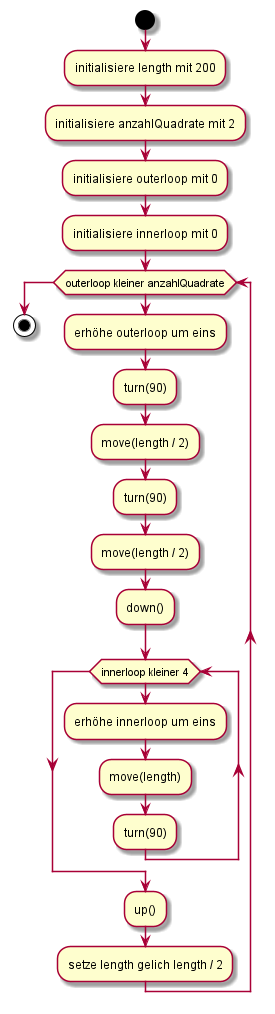
\includegraphics[scale=0.55]{uml/zweiKonzentrischeQuadrate.png}